
%% ICSE 2027 — Research Track submission (double-blind)
%% Format: IEEE two-column conference. Swap the documentclass if ICSE 2027
%% mandates the ACM acmart format (the section files are class-agnostic).
\documentclass[conference]{IEEEtran}
\IEEEoverridecommandlockouts

% ---------- packages ----------
\usepackage{cite}
\usepackage{amsmath,amssymb,amsfonts}
\usepackage{graphicx}
\usepackage{booktabs}
\usepackage{multirow}
\usepackage{array}
\usepackage{algorithm}
\usepackage{algpseudocode}
\usepackage{xcolor}
\usepackage{microtype}
\usepackage[hidelinks]{hyperref}
\usepackage{balance}
\usepackage{xspace}

% ---------- convenience macros (names are PLACEHOLDERS; see ICSE/README.md) ----------
\newcommand{\sys}{\textsc{Arise}\xspace}         % ARISE: Adaptive Retrieval for Incident Support and Explanation
\newcommand{\hit}[1]{Hit@#1}

\begin{document}

% \title{Capability-Gated Agentic Incident Triage:\\
% Matching Live Incidents to Resolved Tickets from Telemetry to the Real World}
\title{ARISE: Adaptive Retrieval for Incident Support and Explanation}

% --- double-blind: anonymized authors ---
%\author{\IEEEauthorblockN{Anonymous Author(s)}
%\IEEEauthorblockA{Submitted for double-blind review, ICSE 2027}}

\maketitle

\begin{abstract}
On-call engineers triage a steady stream of alerts, and their most valuable diagnostic resource is institutional memory: how similar past incidents were diagnosed and resolved. Retrieving the right prior incident is hard, yet existing automated-triage methods are evaluated almost entirely on synthetic fault-injection telemetry under fixed observability assumptions, leaving their effectiveness on real engineer-written incidents largely unknown.
We present \textbf{ARISE}, an adaptive incident-triage framework that retrieves past incidents by fusing dense, lexical, and knowledge-graph retrieval and invokes additional reasoning only when uncertainty justifies its cost, letting one system span regimes from rich telemetry to text-only reports. We evaluate it on three datasets of increasing realism: two new telemetry-to-ticket datasets that pair multi-signal telemetry with incident tickets and per-window labels, and a real-world corpus of 38,642 resolved Apache Jira incidents across 24 projects. On real incidents, under an inferred project-component relevance relation, ARISE retrieves a relevant prior incident in its top five 97\% of the time, improving over dense, lexical, graph, and sampled retrieval-augmented LLM baselines on Hit@5, while capability gating cuts estimated per-window cost by up to 78\% relative to a run-all cascade.
A synthetic-versus-real comparison further shows that ticket-worthiness classification is saturated on injected telemetry (ROC area $1.00$) but only weakly predictable from real, engineer-written ticket text (ROC area $0.57$--$0.60$), where it barely improves on a majority-class baseline. This contrast suggests that the more transferable benchmark target is incident-memory retrieval rather than alert classification alone. We release our datasets, code, evaluation harness, and results.

\end{abstract}

\begin{IEEEkeywords}
incident triage, AIOps, information retrieval, large language models, empirical software engineering
\end{IEEEkeywords}

% === Introduction ===
\section{Introduction}
\label{sec:introduction}

Modern cloud services emit a relentless stream of alerts, and on-call engineers
must decide, often within minutes, which signal a genuine incident and which are
noise~\cite{he2021survey,ghosh2022incidents}. The decision is consequential both
ways: a missed incident becomes an outage, while a flood of low-value pages
erodes trust in the alerting system. What makes an on-call engineer effective is
rarely raw signal-reading; it is \emph{memory}. Most incidents rhyme with one the
team has resolved before, and the fastest path from symptom to fix is to
recognize ``the message-broker outage from last quarter'' and reuse the
diagnosis that worked.

This has motivated a large literature on automated incident triage and
AIOps~\cite{he2021survey,chen2019triage,ghosh2022incidents}, increasingly powered
by large language models~\cite{ahmed2023rootcause,chen2024rcacopilot}. That
literature is evaluated in a strikingly uniform way: faults are scripted into a
demonstration microservice application, telemetry is collected, and a system is
scored on whether it can tell a faulty window from a healthy
one~\cite{chen2025aiopslab}. Reported numbers are high and still improving.

This paper asks whether that is the right thing to measure.

\smallskip
\noindent\textbf{The problem.} We find that the dominant benchmark target is
saturated by construction and does not survive contact with real incidents.
Deciding whether a window warrants a ticket is almost perfectly solvable on
injected faults --- an active fault differs from a healthy baseline by
design --- yet only weakly predictable from the text of real, engineer-written
tickets. On our corpora the same task moves from ROC area $1.00$ to
$0.57$--$0.70$. A strong score on fault-injection data therefore certifies the
dataset, not the method.

Worse, we find that several evaluation choices which are routinely left
implicit change not just the magnitude of a result but its \emph{direction}.
Whether retrieval fusion helps or hurts depends on the size of the corpus it is
measured on. Whether a reported margin is significant depends on whether the
training seed is treated as a source of variance. Whether a method looks best
depends on which of two defensible relevance relations is used. We know these
because each of them reversed or materially altered one of our own conclusions.

\smallskip
\noindent\textbf{What we do.} We run a measurement study across three corpora of
increasing realism: two newly released microservice-telemetry datasets that pair
multi-signal telemetry with incident tickets and per-window labels (Online
Boutique and OTel Demo)\footnote{\url{https://zenodo.org/records/21096887}} and
$38{,}642$ real Apache Jira incidents across 24 projects (World of
Logs~\cite{wang2026worldoflogs}). Throughout we use \sys{}, a retrieval system
that fuses dense, lexical, and knowledge-graph matching behind a cost-aware
controller, as the \emph{instrument}: a strong, realistic baseline whose
behaviour exposes the measurement problems we are studying. Several of our findings
are unflattering to it, which is the point --- the object of study is the
evaluation, not the system.

\smallskip
\noindent\textbf{Contributions.}
\begin{itemize}
  \item \textbf{Evidence that the dominant target does not transfer.}
  Ticket-worthiness classification is saturated on injected faults and only
  weakly learnable on real incidents, while incident-memory retrieval is
  measurable identically on both and does transfer. We also show that our own
  earlier reading of this result was an artifact of a degenerate feature matrix,
  and how a one-line check catches it.

  \item \textbf{A quantification of how much protocol choices move results.}
  The training seed accounts for up to $28\%$ of variance in a headline metric;
  GPU fine-tuning does not reproduce at a fixed seed; the choice of relevance
  relation moves \hit{5} by $0.23$ and reorders methods; and retrieval-fusion
  conclusions \emph{reverse} between a $347$-item and a $38{,}642$-item memory.

  \item \textbf{Two released telemetry-to-ticket datasets} pairing logs,
  metrics, traces, and cluster events with incident tickets and per-window
  labels (26 and 52 fault scenarios), to our knowledge the first public corpora
  coupling telemetry and tickets at this granularity, alongside all code,
  baselines, ablations, and significance
  tests.\footnote{\url{https://zenodo.org/records/21096898}}

  \item \textbf{A protocol for evaluating incident triage}
  (\S\ref{sec:recommendations}), each item tied to a specific way our own
  results would have misled without it.
\end{itemize}

\noindent We report findings that are unfavourable to the instrument as
readily as favourable ones: no evidence-gathering tool in \sys{} has a
measurable benefit, its escalation gates fire roughly $16\times$ more often than
necessary, and its retrieval fusion improves top-five recall while
significantly degrading top-one precision. These are the kinds of result a
system paper is tempted to omit, and the kinds a measurement paper exists to
report.

% === Related Work ===
\section{Related Work}
\label{sec:related}

\noindent\textbf{Incident management and AIOps.} Cloud and microservice operations
generate incident volumes that overwhelm manual on-call triage, motivating a large
AIOps literature~\cite{notaro2021aiops,he2021survey}. Ghosh et al.~\cite{ghosh2022incidents}
document the long detection-to-mitigation pipeline that motivates automation, and
Chen et al.~\cite{chen2019triage} frame \emph{continuous incident triage} as
routing incidents to the correct team. \sys{} reframes this bottleneck as retrieval against a memory of resolved incidents rather than classification.

\noindent\textbf{LLMs for incident diagnosis.} Recent work applies LLMs to root-causing and mitigation: Ahmed et al.~\cite{ahmed2023rootcause}
study LLM-recommended root causes at scale, RCACopilot~\cite{chen2024rcacopilot}
couples diagnostic-data collection with LLM reasoning and matches incidents to
handlers by alert type, and D-Bot~\cite{zhou2024dbot} diagnoses database faults
with LLM agents; AIOpsLab~\cite{chen2025aiopslab} evaluates such agents in
autonomous-cloud settings. \sys{} differs through a capability-gated controller
that runs only the steps the available evidence supports, degrading from full
telemetry to text-only input, and through duplicate-page suppression.

\noindent\textbf{Log analysis and anomaly detection.} A complementary line mines
telemetry directly: Drain~\cite{he2017drain} parses logs into templates, while
DeepLog~\cite{du2017deeplog}, LogAnomaly~\cite{meng2019loganomaly}, and
LogBERT~\cite{guo2021logbert} detect sequential and semantic anomalies, with
standardized benchmarks~\cite{zhu2019logparsing,he2016experience,zhu2023loghub}.
\sys{} consumes parsed telemetry as one capability tier but does not depend on it,
retaining text-only operation when traces and metrics are unavailable.

\noindent\textbf{Retrieval and retrieval-augmented reasoning.} \sys{}'s retriever
fuses dense, sparse, and graph signals. Dense bi-encoders build on
Sentence-BERT~\cite{reimers2019sbert} and the backbones
MiniLM~\cite{wang2020minilm} and MPNet~\cite{song2020mpnet}, with embedding
families E5~\cite{wang2022e5} and BGE/C-Pack~\cite{xiao2024cpack}; sparse retrieval
uses BM25~\cite{robertson2009bm25} and the learned-sparse
SPLADE~\cite{formal2021splade}; cross-encoder re-ranking
follows~\cite{nogueira2019passage}; and we fuse ranked lists with reciprocal rank
fusion~\cite{cormack2009rrf}. DPR~\cite{karpukhin2020dpr}, RAG~\cite{lewis2020rag},
and ReAct~\cite{yao2023react} established the retrieve-then-reason and
reason-and-act paradigms that \sys{}'s evidence-gathering loop and its underlying
LLM~\cite{qwen2024} inherit. Unlike open-ended RAG pipelines, ARISE treats retrieval quality, cost, and evidence availability as first-class evaluation targets, which is important because incident triage sits on a latency-sensitive operational path.

\noindent\textbf{Knowledge graphs and duplicate-incident retrieval.} Knowledge
graphs over incidents and tickets support structured retrieval;
SoftNER~\cite{shetty2022softner} mines them from cloud incidents, informing
\sys{}'s graph retriever. Our ``retrieve the most similar past incident'' framing
also descends from duplicate and similar bug-report
retrieval~\cite{runeson2007duplicate,sun2010duplicate,he2020dccnn}, which \sys{}
extends to operational incidents with telemetry-aware, capability-gated retrieval. This distinction matters because operational incidents may expose structured runtime evidence, while classic duplicate-bug retrieval usually operates only over issue text.

\noindent\textbf{Benchmark systems and data.} Our two collected
microservice-telemetry datasets build on Google's Online
Boutique~\cite{googleboutique} and the OpenTelemetry Demo~\cite{oteldemo} under
controlled Chaos Mesh~\cite{chaosmesh} fault injection; our real-world corpus is
drawn from the World of Logs collection~\cite{wang2026worldoflogs}, with other
large public Jira datasets~\cite{montgomery2022jira} offering complementary issue
data.

% === Background and Motivating Example ===
\section{Background and Motivating Example}
\label{sec:background}

Consider an engineer on call for a microservice application, paged when checkout requests begin to fail. The pressing question is not how to repair the
system from first principles but \emph{what is happening} and \emph{whether it
warrants action}. In a fully instrumented deployment the evidence is rich yet noisy: the cluster reports a message broker's pod unavailable, its consumer services begin logging errors, distributed traces show their requests failing downstream, and an availability alert fires.

The shortcut a seasoned engineer takes is \emph{recognition}: this pattern, a broker outage stalling its consumers and surfacing as checkout failures, has occurred before, and a resolved ticket already records how it was diagnosed and fixed. Retrieving that ticket turns an open-ended investigation into a near-instant analogy, the most direct path from symptom to resolution, provided the past incident can be found. We do not attempt to prove the root cause of the live incident from first principles; instead, we rank historical incidents that provide plausible analogies for human triage.

Two characteristics of operational triage shape our design. First, the \emph{same incident can arrive with vastly different evidence}. The broker failure above may carry logs, metrics, traces, and cluster events; in another team's tracker the identical failure may be a single sentence (``consumers stalled after the broker restarted, backlog growing'') with no telemetry. Yet the task is identical: identify the most relevant resolved incident. A system that depends on complete observability fails precisely when historical knowledge is needed most. Second, an incident is \emph{not instantaneous}: it evolves over a sequence of windows, from early warning signs through active failure to recovery, so treating each window independently produces repeated alerts for one evolving incident.

\smallskip
\noindent\textbf{What an incident is, concretely.} Before introducing notation we
state what the objects are, since the formalism is otherwise easy to read as
abstract. \emph{A memory item is a resolved issue-tracker ticket} written by
engineers in the course of their work. On our real corpus it is a genuine Apache
Jira issue of type \textsc{Bug} with resolution \textsc{Fixed}; the retrievable
document is its summary, description, and the log and stack-trace blocks its
authors pasted into the thread, and there are $38{,}642$ of them. On our
telemetry corpora it is a ticket generated from a deliberately injected fault's
ground truth and rewritten into engineer prose, which is why the link from
observation to ticket there is exact rather than inferred.

\emph{A query is whatever the system is handed at decision time.} In an
instrumented deployment that is a five-minute slice of one service's activity:
its log lines, its CPU, memory and restart series, any firing alerts, the
cluster's pod events, and a sample of distributed-trace spans. In a text-only
deployment it is the incident report itself, with no telemetry at all. The task
is identical in both cases, which is the point.

\smallskip
\noindent\textbf{Problem formulation.}
We formulate incident triage as adaptive retrieval over a time-aware incident memory under heterogeneous evidence. Let
$\mathcal{W}=\{w_1,\ldots,w_n\}$ denote a time-ordered stream of observation
windows, where each window
\[
w_i=(t_i,\mathbf{x}_i,e_i)
\]
is observed at time $t_i$, contains a textual summary $\mathbf{x}_i$, and may
include an arbitrary subset of auxiliary evidence
$e_i\subseteq\{\text{metrics},\text{logs},\text{traces},\text{events}\}$.

The retrieval memory
$\mathcal{M}=\{m_1,\ldots,m_N\}$ consists of previously resolved incidents.
Each incident
\[
m_j=(\mathbf{d}_j,\mathcal{E}_j,\tau_j)
\]
contains its textual description $\mathbf{d}_j$, a set of extracted entities
$\mathcal{E}_j$ (e.g., services, components, error classes, and symptoms), and
its resolution time $\tau_j$. Concretely, $\mathbf{d}_j$ is the ticket text
described above, $\mathcal{E}_j$ is produced offline by a language model reading
only that text (\S\ref{sec:approach-kg}), and $\tau_j$ is the issue's resolution
timestamp. To prevent temporal leakage, only incidents
resolved before the current observation are searchable; for a window observed at
time $t_i$, the eligible memory is
\[
\mathcal{M}_{<t_i}=\{m_j\in\mathcal{M}\mid \tau_j<t_i\}.
\]

In all evaluations, the query incident itself is removed from the searchable memory; for real Jira issues, the query time is the issue creation time and memory eligibility is determined by the candidate issue’s resolution time. Given a window $w_i$, the objective is to retrieve the top-$k$ most relevant
historical incidents from $\mathcal{M}_{<t_i}$ while simultaneously deciding
whether the window warrants an engineer page. Since consecutive windows often belong to the same operational event, the system must additionally associate related windows into one incident so that only one page is issued.

\smallskip
\noindent\textbf{Why windows.} Nothing in the formulation requires discretizing
the stream: $\mathcal{M}_{<t}$ is defined continuously in $t$, and no part of the
retrieval depends on where a window boundary falls. We window because that is the
granularity at which \emph{ground truth exists}. A label states that a competent
engineer would have opened an issue over some interval of activity, and our
synthetic corpora are annotated per five-minute interval; a continuous
formulation would need continuous supervision we cannot obtain. Windowing also
matches how the alerting rules these datasets emulate are themselves evaluated,
and it is what creates the duplicate-page problem the state layer exists to
solve. The windowing is therefore a property of the evaluation, not a commitment
of the method.

% === Approach ===
\section{Approach}
\label{sec:approach}

\sys realizes the task of \S\ref{sec:background} as a capability-aware system
organized around retrieval from the memory of resolved incidents. Two commitments
shape it: \emph{match by analogy}, ranking past incidents by similarity to the
current window and reusing their diagnosis; and \emph{adapt to the evidence each
window carries}, so one system spans conditions from a richly instrumented
deployment to a one-line text report. Figure~\ref{fig:arch} shows the pipeline;
throughout, we return the $k=5$ most similar past incidents for each window.

\begin{figure*}[t]
\centering
\includegraphics[width=.9\textwidth]{figures/arise-architecture.pdf}
\caption{The \sys{} instrument. \circled{1}~Each observation window (rich
telemetry or a bare text report) is profiled into eleven binary capability
flags, from which a deterministic controller assembles a cheap-first plan under
a hard per-window budget. \circled{2}~When the fast path is unconvincing
(numeric triage ${<}\,0.90$ or no confident dense match), the escalation gate
schedules the full hybrid retrieval: dense, sparse, and graph retrievers over a
time-aware memory of resolved tickets, fused by reciprocal rank fusion
($\kappa{=}60$, top-20 per retriever); a second gate triggers query
reformulation when $\mathrm{maxconf}(R)<0.5$. \circled{3}~Bounded
evidence-gathering refines the fused ranking, \circled{4}~a calibrated head
issues the triage and novelty decisions, and \circled{5}~a state layer
suppresses duplicate pages across an incident's windows. Dashed arrows are
offline or asynchronous: the knowledge graph is built once per corpus by LLM
extraction over ticket text, and retrievers see only tickets resolved before
the window's timestamp. The gold card summarizes what we \emph{measure} about
the instrument across five training seeds (\S\ref{sec:results-rq1},
\S\ref{sec:results-rq3}).}
\label{fig:arch}
\end{figure*}

\subsection{Capability Profiling and Gated Planning}
\label{sec:approach-controller}

\sys{} first decides \emph{what to do}, then executes; the decision is driven by a
\emph{capability profile}. A lightweight observer maps a window
$w=(t,\mathbf{x},e)$ to a set of binary capability flags
$\mathcal{C}(w)\subseteq\mathcal{F}$, where $\mathcal{F}$ is a fixed vocabulary of
eleven flags (\textsc{Text}, \textsc{NumericFeatures}, \textsc{OrderedLogs},
\textsc{TraceSummary}, \textsc{ClusterEvents}, \textsc{Metrics},
\textsc{GraphEntities}, and others), each set by a deterministic predicate on the
evidence present. Every reasoning step, or \emph{skill}, declares a requirement
set $\mathrm{req}(s)$ and is admissible for $w$ only when
$\mathrm{req}(s)\subseteq\mathcal{C}(w)$. A deterministic controller composes the
admissible skills into an ordered \emph{plan} $P(w)$, choosing a branch from the
window's role in the incident lifecycle: a quiet pre-fault baseline, an active
fault, a recovery phase, or a continuation of an already-paged incident. Because
inadmissible skills are never scheduled, the system degrades gracefully by
construction: a fully instrumented window yields a plan with numeric triage, all
three retrievers, on-demand evidence requests, and an optional verifier, while a
text-only window drives the identical controller to a compact dense-and-graph plan,
with no code or configuration change.

Planning is also cost-aware. Skills are ordered cheapest first, and the expensive
ones sit behind two \emph{gates} that open only under uncertainty.

\noindent\emph{Confidence.} Both gates read a confidence $c\in[0,1]$, the score a
skill attaches to its own output: for the numeric triage classifier its
calibrated ticket-worthiness probability, and for a retriever the calibrated
probability its logistic head assigns to the window given its best match. We
write
\begin{equation}
\mathrm{maxconf}(R)=\max_{r\in\{\text{dense},\,\text{sparse},\,\text{graph}\}} c_r,
\label{eq:maxconf}
\end{equation}
the largest such confidence over the retrievers that have run. We stress that
$\mathrm{maxconf}$ is \emph{not} the fused score of Eq.~\ref{eq:rrf}: reciprocal
rank fusion produces an unnormalized quantity bounded above by
$3/(\kappa+1)\approx0.049$, which would make a comparison against $0.5$
meaningless. The two live on different scales and are never compared. On the real
corpus the realized $\mathrm{maxconf}$ spans $[0.00,0.57]$ with median $0.42$ and
quartiles $0.36$ and $0.48$, so a $0.5$ threshold sits just above the upper
quartile of the distribution it is applied to.

\noindent\emph{The gates.} A fast pass runs the numeric triage classifier and a
dense lookup. The \emph{escalation gate} schedules the costlier sparse and graph
retrievers and the language-model verifier when this cheap path is unconvincing:
when the numeric triage score falls below $0.90$ or the dense retriever returns no
confident match. A text-only window has no numeric signal to read, so this gate
opens on essentially every window of the real corpus, which is the intended
degraded-mode behaviour. The \emph{reformulation gate} then triggers query
rewriting when $\mathrm{maxconf}(R)<0.5$, signalling that no acceptable precedent
was found; if that persists, the window is flagged novel. Both thresholds are the
components' own operating points, fixed in advance rather than tuned on test
data: $0.5$ is the calibrated ticket-worthy/noise boundary shared by every
retrieval head, and $0.90$ is the numeric classifier's high-confidence commit
point. We report their sensitivity in \S\ref{sec:results-rq3}. A
hard per-window budget bounds the worst case, capping language-model tokens
($10^5$), wall-clock time ($90$\,s), monetary cost (\$$0.50$), and total skill
invocations ($12$); an exhausted budget returns the best partial result. Because
almost every skill reads precomputed signals, the only steps that call a language
model at decision time are the gated verifier and reformulator.
Algorithm~\ref{alg:window} summarizes the per-window procedure.

\begin{algorithm}[t]
\caption{Per-window triage in \sys{}}
\label{alg:window}
\small
\begin{algorithmic}[1]
\Require window $w=(t,\mathbf{x},e)$; memory $\mathcal{M}$; budget $B$
\Ensure top-$k$ matches $R$; triage decision; incident id
\State $\mathcal{C}\gets \textsc{Capabilities}(w)$ \Comment{evidence profile}
\If{$\textsc{SuppressedByState}(w)$}
  \State \Return suppressed page with inherited incident id
\EndIf
\State $P\gets \textsc{Plan}(\textsc{Branch}(w),\,\mathcal{C})$ \Comment{admissible, cheap-first}
\State $c\gets \textsc{NumericTriage}(w)$ if $\textsc{Numeric}\!\in\!\mathcal{C}$;\;\; $R_d\gets \textsc{Dense}(w,\mathcal{M}_{<t})$
\If{$c<0.90$ \textbf{ or } $|R_d|<1$} \Comment{escalation gate}
  \State $R\gets \textsc{RRF}\big(\textsc{Dense},\textsc{Sparse},\textsc{Graph};\,\mathcal{M}_{<t}\big)$
  \If{$\mathrm{maxconf}(R)<0.5$} \Comment{Eq.~\ref{eq:maxconf}, not Eq.~\ref{eq:rrf}}
    \State $R\gets \textsc{Reformulate}(w,\mathcal{M}_{<t})$
  \EndIf
  \If{telemetry available \textbf{ and } still uncertain}
    \State $R\gets \textsc{RerankByEvidence}\big(R,\textsc{Gather}(w)\big)$
  \EndIf
\Else
  \State $R\gets R_d$
\EndIf
\State $p\gets \sigma(\boldsymbol{\beta}^{\top}\mathbf{z}+b)$;\;\; decision $\gets [\,p\ge 0.5\,]$
\State id $\gets \textsc{StateUpdate}(w,R_1)$;\;\; \Return $R_{1:k}$, decision, id
\end{algorithmic}
\end{algorithm}

\noindent\textbf{Deterministic control.}  ARISE uses adaptive tool selection but keeps
control deterministic. This preserves reproducibility, bounded cost,
and auditability: each action follows an explicit capability rule and
budget rather than an open-ended model loop. Language-model calls
are therefore limited to gated verification and reformulation steps.

\subsection{Hybrid Memory Retrieval}
\label{sec:approach-retrieval}

The core of \sys{} ranks the eligible memory $\mathcal{M}_{<t}$ against a window
by fusing three complementary measures of similarity, none reliable in isolation.
The \emph{dense} retriever embeds window and ticket text with a fine-tuned
bi-encoder $\phi$ and scores by cosine similarity,
\begin{equation}
s_{\text{dense}}(w,m)=\cos\!\big(\phi(\mathbf{x}_w),\,\phi(\mathbf{d}_m)\big).
\end{equation}
We fine-tune a compact ($384$-dimensional) MiniLM bi-encoder~\cite{wang2020minilm,reimers2019sbert}
with a multiple-negatives ranking loss~\cite{karpukhin2020dpr}: each
window is paired with its gold ticket as a positive against the rest of the batch,
two hard negatives mined by a lexical retriever~\cite{robertson2009bm25}, and one
random negative, teaching it to separate genuinely related incidents from those
that are merely lexically similar. The dense view captures paraphrase and semantic
overlap but blurs exact tokens; the \emph{sparse} retriever, a learned sparse
lexical model~\cite{formal2021splade}, restores that precision by matching the
literal identifiers, error codes, and component names that distinguish otherwise
similar incidents.

The third view is a \emph{knowledge-graph} retriever that captures structural
rather than surface resemblance (\S\ref{sec:approach-kg}). Each retriever proposes
its top $20$ candidates, and we merge the three ranked lists with reciprocal rank
fusion~\cite{cormack2009rrf}. Writing $\mathrm{rank}_r(m)$ for the position of
incident $m$ in retriever $r$'s list, the fused score is
\begin{equation}
s_{\text{fuse}}(m)=\sum_{r\in\{\text{dense},\,\text{sparse},\,\text{graph}\}}
\frac{1}{\kappa+\mathrm{rank}_r(m)},\qquad \kappa=60,
\label{eq:rrf}
\end{equation}
where an incident contributes nothing from a retriever that does not rank it. A final composition step sharpens the head of the list, anchoring on the dense retriever's strongest candidates and promoting those the sparse and graph retrievers independently corroborate. One view's blind spot is thus covered by another's strength, the central reason the fused ranker beats every constituent
alone (\S\ref{sec:results}).

\subsection{Knowledge-Graph Construction and Retrieval}
\label{sec:approach-kg}

We build the knowledge graph once, offline, from the resolved tickets in memory. For each ticket we prompt a lightweight language model
(\texttt{gpt-4o-mini}) to emit a structured fact set: the affected services and
components, any canonical error classes (for example \textsc{OOMKilled} or
\textsc{ConnectionRefused}), a one-sentence root cause, a one-sentence fix with a
coarse fix type, and a short list of observable symptoms. These facts are
materialized as a typed property graph with seven node labels (\textsc{Incident},
\textsc{Service}, \textsc{Component}, \textsc{ErrorClass}, \textsc{RootCause},
\textsc{Fix}, \textsc{Symptom}) and six labelled relations; shared entities are
deduplicated, so two incidents that touch the same component or raise the same
error class are linked through it, encoding the structural neighbourhoods that
recur across an operational history.

At query time the same extraction runs on the window (or a fast rule-based
extractor when no language model is configured), and we score each visible
incident by typed entity overlap. With $A_\theta(\cdot)$ the set of entities of
type $\theta$ for a window or incident, the graph score is a weighted sum of
overlaps,
\begin{equation}
s_{\text{graph}}(w,m)=\sum_{\theta}\lambda_\theta\,
\big|A_\theta(w)\cap A_\theta(m)\big|,
\end{equation}
with weights that reflect each signal's diagnostic value: an exact error class is
weighted most heavily ($\lambda_{\text{error}}=3.0$), followed by the affected
service ($2.0$) and component ($1.5$), while symptoms, which recur across many
unrelated incidents, contribute least ($1.0$). The score is a single graph query
that enforces time-aware visibility directly: an incident is eligible only if
its resolution timestamp precedes the window's.

\subsection{Evidence-Grounded Refinement}
\label{sec:approach-react}

When a window carries rich telemetry but the fused ranking remains uncertain,
\sys{} does what an engineer would: it gathers more evidence before committing.
Following the reason-and-act paradigm~\cite{yao2023react}, it issues a few targeted
requests, each returning one compact piece of evidence rather than a verdict
(cluster events, an extended trace slice, pod-level metrics, or past incidents from
the same fault family), then re-ranks candidates by how well each description agrees
with the gathered evidence. The loop is bounded: repeated identical requests are refused,
and the per-window budget caps the total number of calls. On a text-only window
these requests are never scheduled, so the step is a safe pass-through that returns
the fused ranking unchanged.

\smallskip
\noindent\textbf{A representative trajectory.} On a telemetry-rich active-fault
window (a cart service degraded by a failing Redis dependency), the cheap path
fires with a thin margin: two precedents, a cache outage and a memory leak, score
almost equally. \sys{} escalates to the sparse and graph retrievers, requests pod
events and metrics, observes a cache-pod restart and memory saturation alongside
the latency spike, and re-ranks the corroborated cache-dependency precedent to
rank one, stopping below budget while the state layer folds the window into the
ongoing incident.

\subsection{Triage, Novelty, and Incident-Aware Paging}
\label{sec:approach-state}

The retrieval evidence also drives the paging decision. A lightweight logistic
model combines the available cheap signals, the numeric triage classifier's score
where instrumentation exists and the confidence of the best retrieval match, into
a ticket-worthiness probability $p=\sigma(\boldsymbol{\beta}^{\top}\mathbf{z}+b)$,
and the window is judged ticket-worthy when $p\ge 0.5$; on text-only incidents,
which lack a telemetry classifier, the decision rests on retrieval confidence
alone. A window is flagged \emph{novel}, signalling a failure mode with no
precedent in memory, when no source is confident: the disjunction of a low maximum
retriever confidence, a verifier judgement of novelty when the verifier ran, and an
optional learned novelty score. We treat novelty detection as an auxiliary signal rather than as a fully validated claim on real data, because the text-only real corpus does not provide reliable labels for no-precedent incidents.

Because a single incident unfolds across many windows, paging on each would bury
the on-call engineer. \sys{} keeps a per-service ring buffer of its last twelve
decisions and suppresses a duplicate when a window repeats a recently paged incident
(same top-ranked precedent and fault family within a three-window lookback, no
recovery window between), letting it inherit that incident's identifier. Consecutive
windows of one fault thus fold into a single incident, and the system approaches one
page per incident, not one per window (\S\ref{sec:results}).

The optional language-model verifier, which re-examines a borderline match in natural language,
is itself capability-gated: enabled where calibration shows it helps, disabled where
it hurts; on real engineer-written incidents we find it net-negative and switch it
off. Treating whether an expensive reasoning step helps in a given setting as just
another capability is, we argue, much of what keeps one system robust across very
different evidence regimes.

% === Datasets ===
\section{Datasets}
\label{sec:datasets}

A faithful evaluation must cover the range a deployed system faces: from richly instrumented services with logs, metrics, and traces down to bare, text-only reports. We therefore use three datasets along this realism spectrum (Table~\ref{tab:datasets}). The first two we \emph{collect and release}: instrumented microservice systems under controlled fault injection, pairing multi-signal telemetry with incident tickets and exact per-window labels. The third we \emph{reuse}: a large corpus of real, engineer-written Apache Jira incidents testing whether methods tuned on synthetic data hold up in the field. The synthetic datasets support exact window-to-ticket evaluation and telemetry-based gating; the real corpus supports large-scale text-only retrieval under noisier, inferred relevance labels.

\begin{table}[t]
\centering
\caption{The three evaluation datasets, spanning fully instrumented synthetic
incidents to real, text-only ones. \emph{Memory} is the pool of past incidents
available for retrieval; \emph{test windows} are the held-out queries used in
\S\ref{sec:results}.}
\label{tab:datasets}
\footnotesize
\setlength{\tabcolsep}{4pt}
\begin{tabular}{lccc}
\toprule
 & Online Boutique & OTel Demo & World of Logs \\
\midrule
Origin           & collected (ours) & collected (ours) & reused~\cite{wang2026worldoflogs} \\
Evidence         & full telemetry   & full telemetry   & text only \\
Scale            & 11 services      & 17 svc.\ + Kafka & 24 projects \\
Fault scenarios  & 26 families      & 52 scenarios     & real incidents \\
Memory incidents & 347              & 147              & 38{,}642 \\
Test windows     & 1{,}008          & 247              & 13{,}388 \\
Split            & by family        & by family        & leave-domain-out \\
\bottomrule
\end{tabular}
\end{table}

\subsection{Collected Telemetry Datasets}
\label{sec:datasets-synthetic}

\begin{figure}[t]
\centering
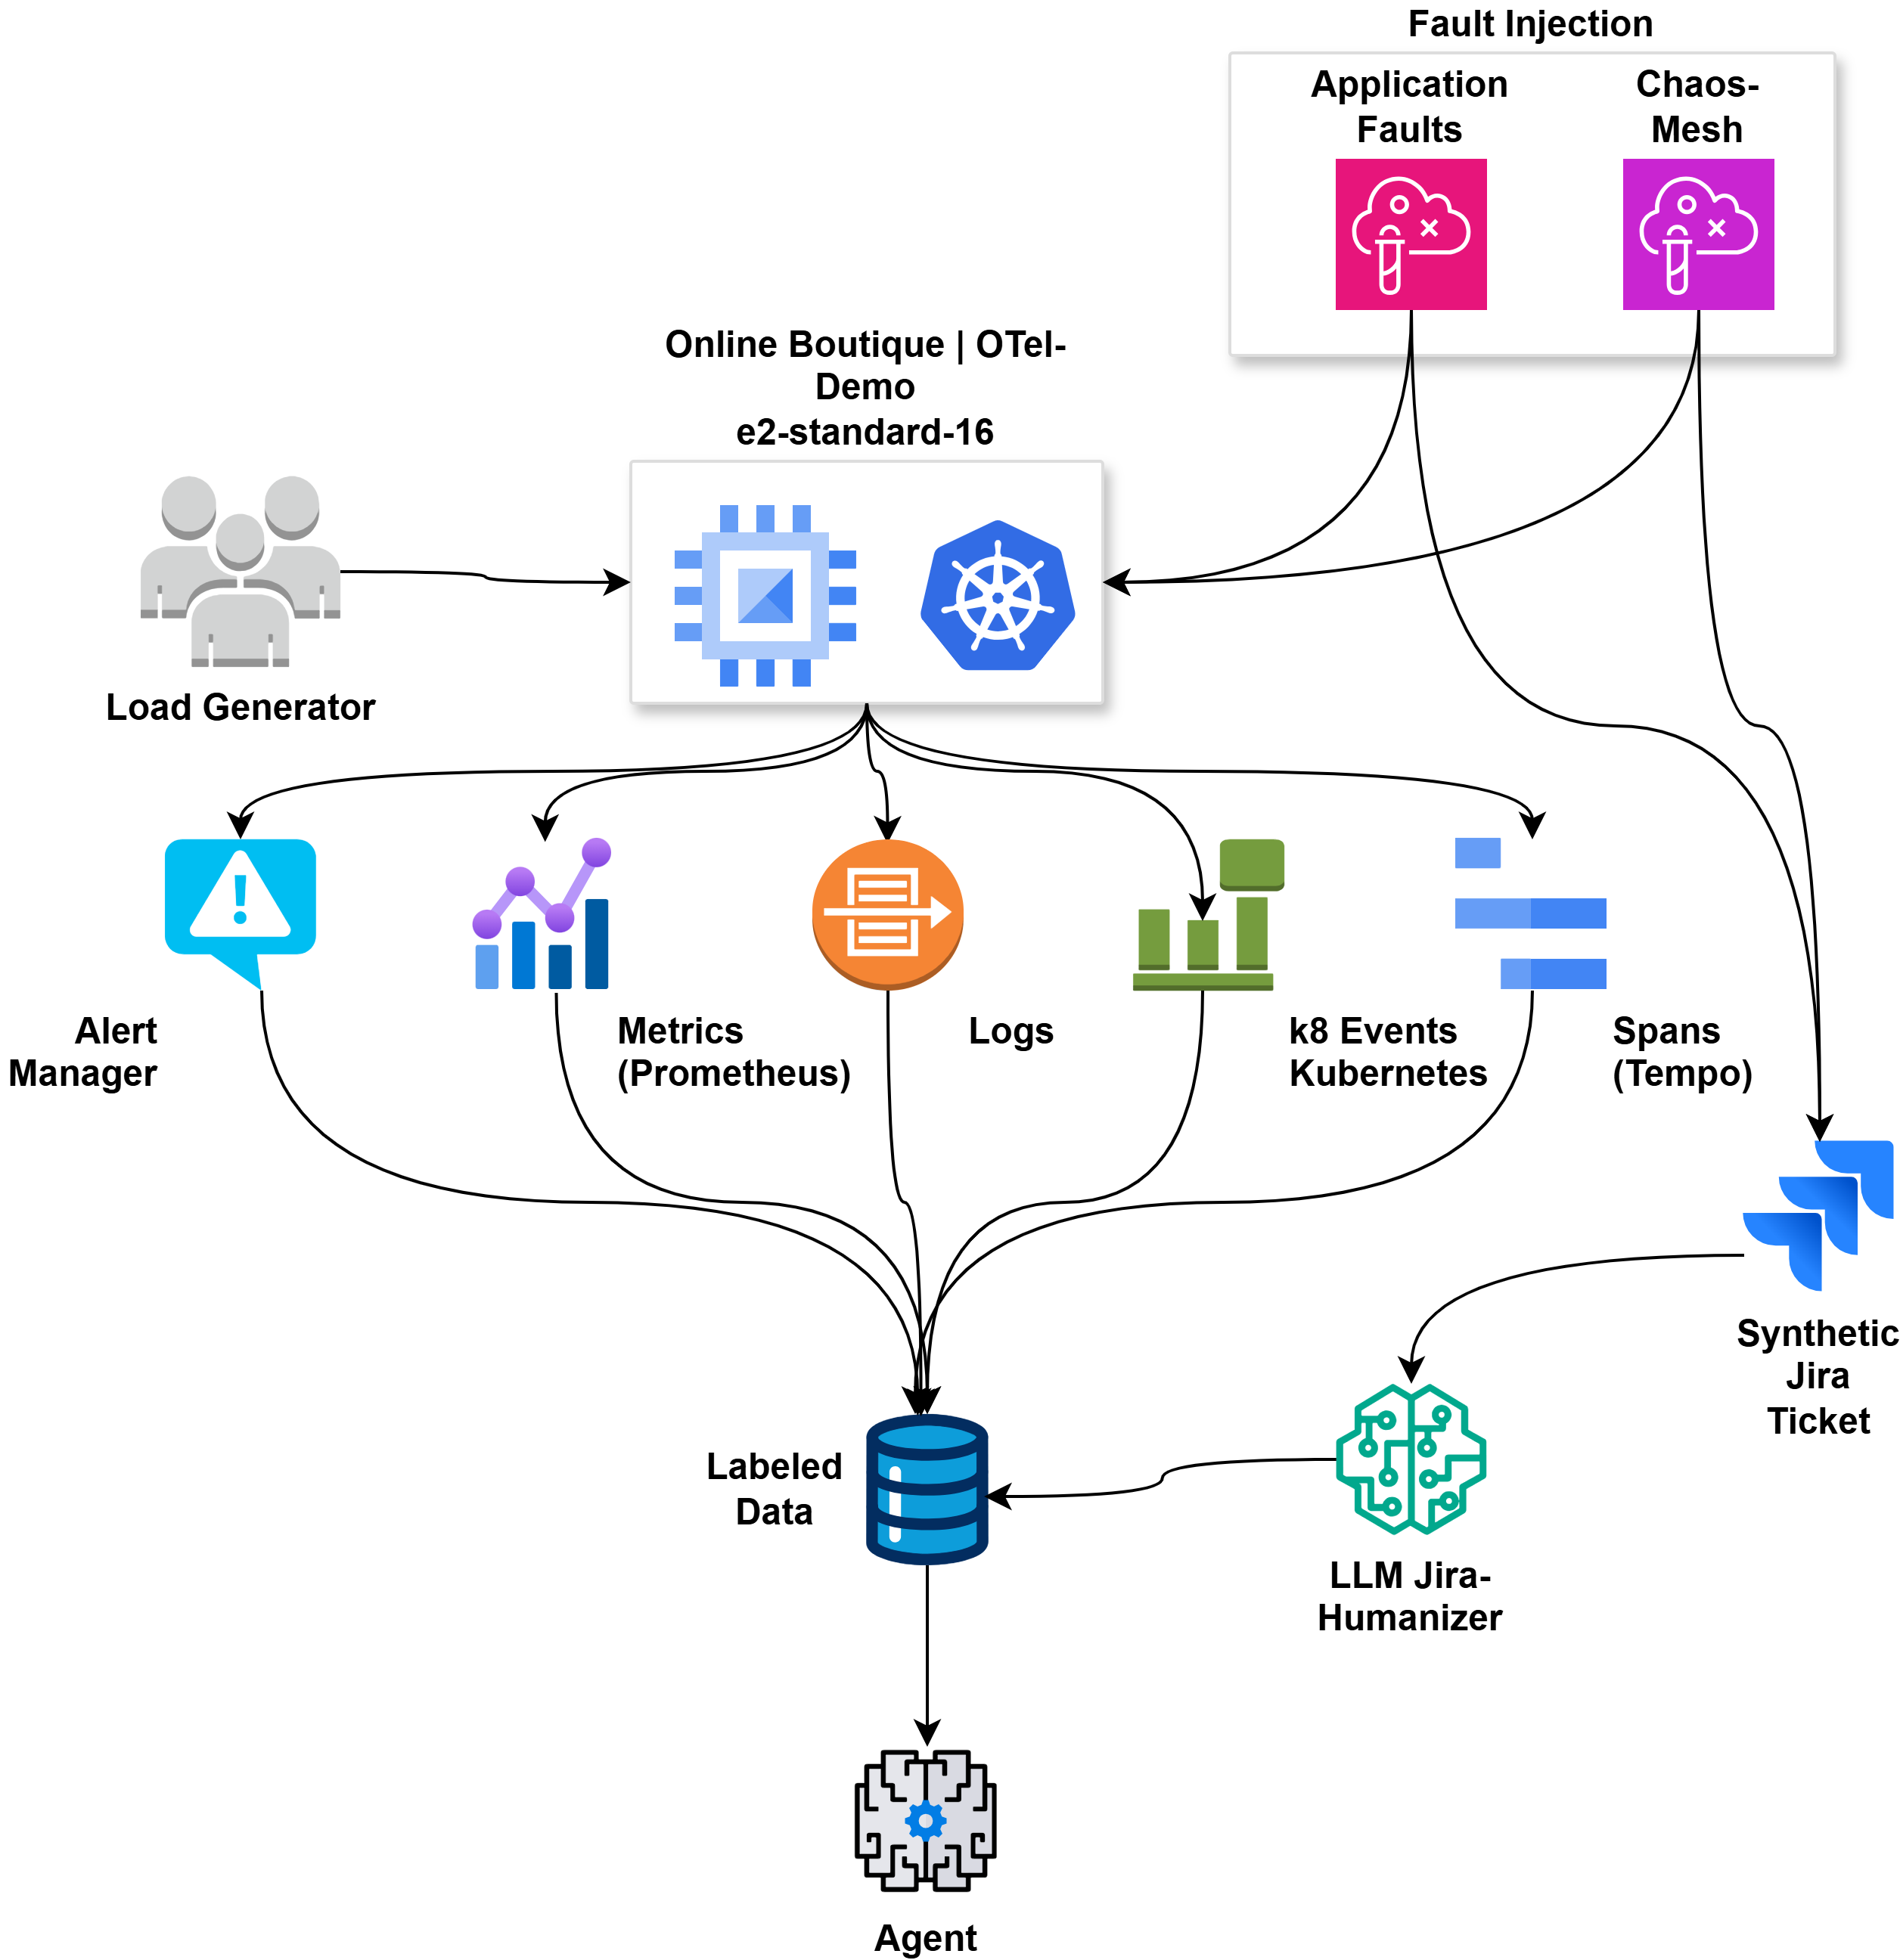
\includegraphics[width=.95\columnwidth]{figures/data-collection.png}
\caption{Data-collection pipeline for the two telemetry datasets. A load
generator exercises an open-source microservice application in Kubernetes while
controlled faults (application-level failures and chaos-engineering network
faults) are injected. The resulting alerts, metrics, logs, cluster events, and distributed-trace spans are captured per window, paired with a synthetic incident ticket (rewritten into engineer voice by a language model) as the retrieval target. The triage system consumes the labelled result.}
\label{fig:collection}
\end{figure}

Both datasets come from a single collection pipeline (Figure~\ref{fig:collection}).
We deploy an open-source microservice application in a Kubernetes cluster
instrumented with a standard observability stack (Prometheus for metrics, Tempo
for distributed traces, and Loki for logs), drive it with a synthetic load
generator, and inject faults under controlled, fully labelled conditions. The
unit of collection is a \emph{scenario}: one fault, injected for a fixed
duration, with its ground truth declared in advance. Each scenario produces three
consecutive \emph{observation windows} (a fault-free baseline just before the
fault, the active fault itself, and a recovery phase after it is cleared), and we
label every window with one of three classes: \textbf{ticket-worthy} (a real
engineer would open an issue), \textbf{borderline} (recovering or marginal), or
\textbf{noise} (normal operation). A window, a short slice of one service's
activity (5 minutes), is the atomic input to the triage system.

For each window we archive everything the platform recorded: the service's logs,
its CPU, memory, and restart series with any firing alerts, the cluster's events
and pod state, and a sample of distributed traces. When a scenario warrants
attention, we generate the incident ticket and rewrite it with a language model
into natural, engineer-voice prose, so the memory reads like real filed tickets;
this ticket is the retrieval target. Because we control the
injection, the window--ticket link is \emph{exact ground truth} rather than
inferred. We also record realistic near-misses (a service stressed but never
failing, warranting no page) and \emph{orphan} faults (genuine ticket-worthy
failures for which no ticket is filed, so a page-worthy window has no precedent in
memory). The near-misses separate a useful triage system from one that pages
constantly; the orphans test whether it recognizes an incident from telemetry
rather than only when a matching ticket exists.

\textbf{Online Boutique}~\cite{googleboutique} is an eleven-service e-commerce demo
spanning five languages; its 26 fault families include hard service outages (e.g., scaling a service to zero replicas), latency and resource-pressure
degradations such as slow memory and connection leaks, pod restarts, network
faults injected with a chaos-engineering tool~\cite{chaosmesh} (partitions, packet
loss, DNS failures), and deployment churn. \textbf{OpenTelemetry
Demo}~\cite{oteldemo} adds architectural distance:
seventeen services in twelve languages, organized around a Kafka message bus with
asynchronous downstream consumers. Its 52 scenarios extend from single-service faults (triggered through the application's built-in failure switches) to Kafka-specific failures such as broker outages and consumer lag with no Online Boutique analogue, and on to concurrent and cascading multi-fault episodes. Together the two contribute roughly $6{,}700$ and $1{,}600$ labelled
windows and tens of gigabytes of raw telemetry, which we release as self-contained
archives. Within each dataset we hold out whole fault families for testing, so test
windows never come from a scenario seen during training.

\subsection{Real-World Incidents: World of Logs}
\label{sec:datasets-wol}

To see whether a method survives contact with reality, we turn to the \emph{World
of Logs} collection~\cite{wang2026worldoflogs}, a public archive of logs and issue reports
mined from online software-engineering sources, including public Jira trackers.
This dataset is not our contribution; we derive an evaluation slice from its Apache Jira issues. We select 24 of its
distributed-systems projects (message brokers, datastores, stream processors,
the Hadoop ecosystem, and others), which together provide a memory of $38{,}642$
resolved bug reports to retrieve from and $78{,}140$ incident queries to triage.
Each query receives the same three labels as our synthetic data, assigned
automatically from the ticket's type and final resolution: a fixed bug is
ticket-worthy, an engaged-but-inconclusive outcome is borderline, and a rejected
or non-bug issue is noise.

This corpus is deliberately the hardest of the three, for two reasons. It is
\emph{text only}: authentic, terse, engineer-written descriptions with no
telemetry whatsoever, exactly the degraded regime to which our controller must
fall back. And we evaluate it under a \emph{leave-domain-out} split, holding out
two entire project families (a message broker and a database engine, $13{,}388$
incidents) so the system must match incidents in projects it never saw while training. 

The counts serve different roles. The 78,140 Jira issues form the labelled triage pool before the held-out-domain split. Table I reports the 13,388 held-out issues used as test windows for end-to-end triage. Retrieval metrics are computed only on held-out fixed-bug queries that have at least one eligible past match under the inferred relation; this yields 5,150 retrieval queries in Table II. Borderline and noise issues are retained for triage evaluation but excluded from Hit@k and MRR because they have no relevant prior incident by construction.

Real incidents come with no manually curated answer key linking each query to the past ticket that would best support triage, so we use an inferred matching relation: a query and a past ticket match when they share a project and at least one software component, with a stricter variant that also requires overlapping symptom terms. We report retrieval quality under both relations and, because inferred labels deserve scrutiny, separately validate them with an LLM-as-judge check (\S\ref{sec:results}). Only genuine bug reports have matches; borderline and
noise queries have none by construction and are excluded from the retrieval
measurements.

\smallskip
\noindent\textbf{Component metadata is load-bearing, so we characterize it.}
Because the relation is defined on the \texttt{project} and \texttt{components}
fields, the quality and coverage of those fields bound what the metric can mean.
Across all $78{,}140$ issues, $75.3\%$ carry at least one component ($80.5\%$ on
the test split); most carry exactly one ($48{,}394$ issues) or two ($8{,}935$).
Vocabularies are project-local and very uneven, from $205$ distinct components in
Camel to $9$ in IMPALA, and they are not a clean taxonomy: alongside subsystem
names they include release numbers such as \texttt{10.3} and \texttt{2.2.1}, so
two issues can share a ``component'' only by sharing a version.

This directly conditions the evaluation, and we state the consequence plainly
rather than leaving it to be inferred from a table. Of the $6{,}773$ held-out
ticket-worthy queries, $1{,}621$ ($23.9\%$) carry no component at all and
therefore have no gold match by construction. The retrieval results in
\S\ref{sec:results} are computed on the remaining $5{,}150$, and the strict
relation reduces this further to $4{,}362$. Our real-corpus retrieval numbers are
thus conditioned on issues whose authors filled in component metadata, a
non-random three quarters of ticket-worthy issues, and they should be read as
describing that subpopulation rather than all real incidents.

% === Experimental Setup ===
\section{Experimental Setup}
\label{sec:setup}

\subsection{Research Questions}
\label{sec:setup-rqs}

Our evaluation is organized around four questions:

\begin{itemize}
  \item[\textbf{RQ1}] \textbf{(Retrieval).} How accurately can a live incident be
  matched to the most similar resolved incident in memory, and does fusing dense,
  lexical, and graph retrieval outperform each in isolation, as well as strong
  prior-art and LLM-based retrievers?
  \item[\textbf{RQ2}] \textbf{(End-to-end triage).} Does the capability-gated
  system retrieve effectively end to end, and does the \emph{same} system hold up
  as the available evidence degrades from full telemetry to text alone?
  \item[\textbf{RQ3}] \textbf{(Cost of adaptive execution).} What does the system's
  capability gating buy? How much triage cost does it save relative
  to running every step on every window, at equal accuracy, and which components
  carry the result?
  \item[\textbf{RQ4}] \textbf{(Synthetic vs.\ real).} How do triage and retrieval
  behave on synthetic versus real incidents, and what does the contrast reveal
  about where the difficulty lies?
\end{itemize}

\subsection{Systems and Baselines}
\label{sec:setup-baselines}

We compare our hybrid retriever and full system against three groups of baselines,
all evaluated under an identical memory, time-aware visibility, and gold contract.

\noindent\emph{Constituent retrievers.} To show fusion exceeds the sum of its parts, we report our fine-tuned dense
bi-encoder and our knowledge-graph retriever on their own, alongside the full
hybrid that fuses them with a learned sparse retriever.

\noindent\emph{Prior-art retrieval.} We add widely used, off-the-shelf retrievers
applied zero-shot: three strong dense embedding models (BGE, E5, and
MPNet)~\cite{xiao2024cpack,wang2022e5,song2020mpnet}, classical lexical search
(TF--IDF and BM25~\cite{robertson2009bm25}), and a cross-encoder
re-ranker~\cite{nogueira2019passage} applied over the dense candidates.

\noindent\emph{Retrieval-augmented LLM.} As a contemporary comparison,
an instruction-tuned language model (Qwen2.5-7B~\cite{qwen2024}) re-ranks the
dense top candidates per query; following common practice, we run it on a fixed
500-incident sample per dataset.

\noindent\emph{Triage classifiers.} For the triage decision (RQ4) we additionally
compare standard classifiers over the numeric telemetry features (gradient-boosted
trees, random forests, and logistic regression) wherever such features exist.

\subsection{Metrics}
\label{sec:setup-metrics}

We measure two capabilities separately. \emph{Retrieval} is scored with
Hit@$k$ (the correct prior incident appears in the top $k$, for
$k\in\{1,5\}$) and mean reciprocal rank (MRR), averaged over queries that have
at least one ground-truth match; on the real dataset we report both the coarse
and strict matching relations of \S\ref{sec:datasets-wol}. \emph{Triage} is a
calibrated classification problem, so beyond accuracy we report the areas under the precision--recall and ROC
curves, and expected calibration error. We also report pages per incident, capturing whether duplicate alerts are
suppressed. Finally,
\emph{cost} is measured per window as wall-clock time and language-model token
usage, relative to a counterfactual cascade that runs every step on every window.

\subsection{Protocol and Implementation}
\label{sec:setup-protocol}

\noindent\emph{Splits.} The synthetic datasets are split by holding out whole
fault families, and the real dataset by holding out two entire project domains
(\S\ref{sec:datasets}); all numbers are reported on the held-out test split.

\noindent\emph{Statistics.} Every reported difference uses a paired bootstrap
($1{,}000$ resamples, $95\%$ confidence intervals) in which the same resampled
windows are scored for both systems, preserving per-window correlation; a
difference is significant when its interval excludes zero. Because we run many comparisons, we control the false-discovery rate across the
test family with the Benjamini--Hochberg procedure and report corrected $q$-values.

\noindent\emph{Where every label comes from.} No label in this paper is produced
by a human annotator, and we state that plainly rather than leaving it to be
inferred. The synthetic triage labels are assigned by construction from the fault
injector: a window inside an injected fault is ticket-worthy, a pre-fault window
is noise, a recovery window is borderline. The real triage labels are derived
mechanically from Jira fields, as described in \S\ref{sec:datasets-wol}. The real
relevance labels are the rule-inferred relations of \S\ref{sec:datasets-wol}. A
language model is used in exactly two places, neither of which produces a
benchmark label: it rewrites synthetic tickets into engineer prose, and it
extracts graph entities offline.

\noindent\emph{Gold validation.} Because the real dataset's matches are inferred
rather than human-labelled, we probe them with an LLM-as-judge. We sample $300$
held-out queries that have a gold match; for each we form two pairs, the query
against a randomly chosen gold match and the query against a memory item sampled
uniformly from outside its gold set, and ask Qwen2.5-7B-Instruct for a single
integer: \emph{``Rate how relevant a past ticket is to a current incident
window\ldots\ 5 = clearly the same or related issue, 1 = unrelated.''} We parse
the first digit of the reply, giving $600$ judgements under greedy decoding at a
fixed seed. We report the gold-versus-control gap, and, because it qualifies the
result, also the fraction of gold matches the judge rates highly
(\S\ref{sec:results-rq4}). The control is sampled uniformly and is therefore an
easy negative; we treat this check as exploratory evidence that the labels carry
signal, not as a substitute for human judgement.

\noindent\emph{Implementation.} The dense retriever is a compact MiniLM
bi-encoder fine-tuned for five epochs with hard negatives mined by lexical search;
the hybrid fuses each retriever's top candidates by reciprocal rank fusion. Graph
entities are extracted from tickets by a small language model and matched by
entity overlap. The retrieval-augmented and judge models run offline with
deterministic (greedy) decoding. Every experiment uses a fixed random seed, and
full configurations and seeds are released with the artifact.

\noindent\emph{Compute environment.} All experiments ran on the Trillium cluster, administered by the Digital
Research Alliance of Canada.\footnote{\url{https://alliancecan.ca}} Each training
and sampling job used a single NVIDIA H100 GPU (80\,GB) with up to 24 CPU cores
and the node's per-GPU share of host memory.

% === Results ===
\section{Results}
\label{sec:results}

\subsection{RQ1: Retrieval Quality}
\label{sec:results-rq1}

Table~\ref{tab:retrieval} reports retrieval quality across all three datasets.
Two findings stand out. First, a retriever fine-tuned on the task far
outperforms strong off-the-shelf methods: our dense bi-encoder beats every
zero-shot dense embedder, classical lexical search, a cross-encoder re-ranker,
and a retrieval-augmented LLM on all three datasets: on real incidents it reaches \hit{5}~$0.91$ against $0.83$--$0.87$ for the best baselines.
The retrieval-augmented LLM, re-reading the same candidates, never surpasses it:
the gains come from domain-adapted retrieval, not a general reader.

\begin{table*}[t]
\centering
\caption{Retrieval quality on the held-out test set: Hit@1, Hit@5, and mean
reciprocal rank (MRR) under the coarse matching relation, averaged over the $n$ test
queries that have a ground-truth match. Best per column in \textbf{bold}. Our
fine-tuned dense retriever leads every zero-shot baseline and the
retrieval-augmented LLM on Hit@5 across all three datasets; hybrid fusion
additionally tops Hit@5 and MRR on the large real-world corpus (World of Logs),
where its Hit@5 gain over the dense retriever and the strongest baselines is
statistically significant (paired bootstrap, Benjamini--Hochberg $q<0.05$;
Fig.~\ref{fig:forest}). On the small synthetic corpora the dense retriever alone is
tied with or ahead of fusion.}
\label{tab:retrieval}
\footnotesize
\setlength{\tabcolsep}{4pt}
\begin{tabular}{l ccc ccc ccc}
\toprule
& \multicolumn{3}{c}{Online Boutique ($n{=}331$)}
& \multicolumn{3}{c}{OTel Demo ($n{=}119$)}
& \multicolumn{3}{c}{World of Logs ($n{=}5{,}150$)} \\
\cmidrule(lr){2-4}\cmidrule(lr){5-7}\cmidrule(lr){8-10}
Method & \hit{1} & \hit{5} & MRR & \hit{1} & \hit{5} & MRR & \hit{1} & \hit{5} & MRR \\
\midrule
\multicolumn{10}{l}{\emph{Prior art, zero-shot}}\\
\quad BGE (dense)          & 0.172 & 0.341 & 0.244 & 0.387 & 0.664 & 0.508 & 0.623 & 0.829 & 0.710 \\
\quad E5 (dense)           & 0.154 & 0.314 & 0.224 & 0.479 & 0.538 & 0.509 & 0.639 & 0.838 & 0.725 \\
\quad MPNet (dense)        & 0.202 & 0.375 & 0.278 & 0.227 & 0.630 & 0.404 & 0.644 & 0.834 & 0.725 \\
\quad TF--IDF (lexical)    & 0.127 & 0.372 & 0.231 & \textbf{0.521} & 0.613 & 0.563 & 0.521 & 0.766 & 0.626 \\
\quad Cross-encoder rerank & 0.103 & 0.296 & 0.182 & 0.311 & 0.580 & 0.441 & 0.686 & 0.874 & 0.766 \\
\multicolumn{10}{l}{\emph{Retrieval-augmented LLM}}\\
\quad Qwen2.5-7B           & 0.239 & 0.344 & 0.293 & 0.370 & 0.639 & 0.501 & 0.710 & 0.856 & 0.778 \\
\multicolumn{10}{l}{\emph{Ours}}\\
\quad Dense bi-encoder     & \textbf{0.432} & \textbf{0.634} & \textbf{0.512} & 0.445 & \textbf{0.681} & 0.549 & \textbf{0.856} & 0.905 & 0.874 \\
\quad Knowledge graph      & 0.396 & 0.465 & 0.420 & 0.067 & 0.412 & 0.227 & 0.083 & 0.308 & 0.152 \\
\quad Hybrid fusion        & 0.414 & 0.559 & 0.461 & 0.513 & 0.672 & \textbf{0.568} & 0.839 & \textbf{0.970} & \textbf{0.897} \\
\bottomrule
\end{tabular}
\end{table*}

Second, the value of \emph{fusion} depends on the setting. On the large,
heterogeneous real corpus, fusing the dense, sparse, and graph retrievers lifts
\hit{5} from $0.91$ to $0.97$, placing the correct prior incident in the top
five $97\%$ of the time, at \hit{1}~$0.84$ and MRR~$0.90$. This gain is large and
statistically significant: against the dense retriever the paired-bootstrap
difference is $+0.065$ ($95\%$ CI $[+0.058,+0.073]$), and against the strongest
baselines it ranges from $+0.12$ (the LLM) to $+0.14$ (zero-shot dense), all with
Benjamini--Hochberg $q\approx 0$. On the two small synthetic corpora, by
contrast, the fine-tuned dense retriever is already so strong that fusion does
not help, and on Online Boutique it is slightly worse ($-0.076$, $q=0.03$):
when one retriever dominates a small memory, blending in weaker signals only adds
noise. Fusion's advantage thus \emph{emerges with scale and diversity}, precisely
the conditions of real operations. Figure~\ref{fig:forest} summarizes every
pairwise comparison with its bootstrap confidence interval and significance.

\begin{figure}[t]
\centering
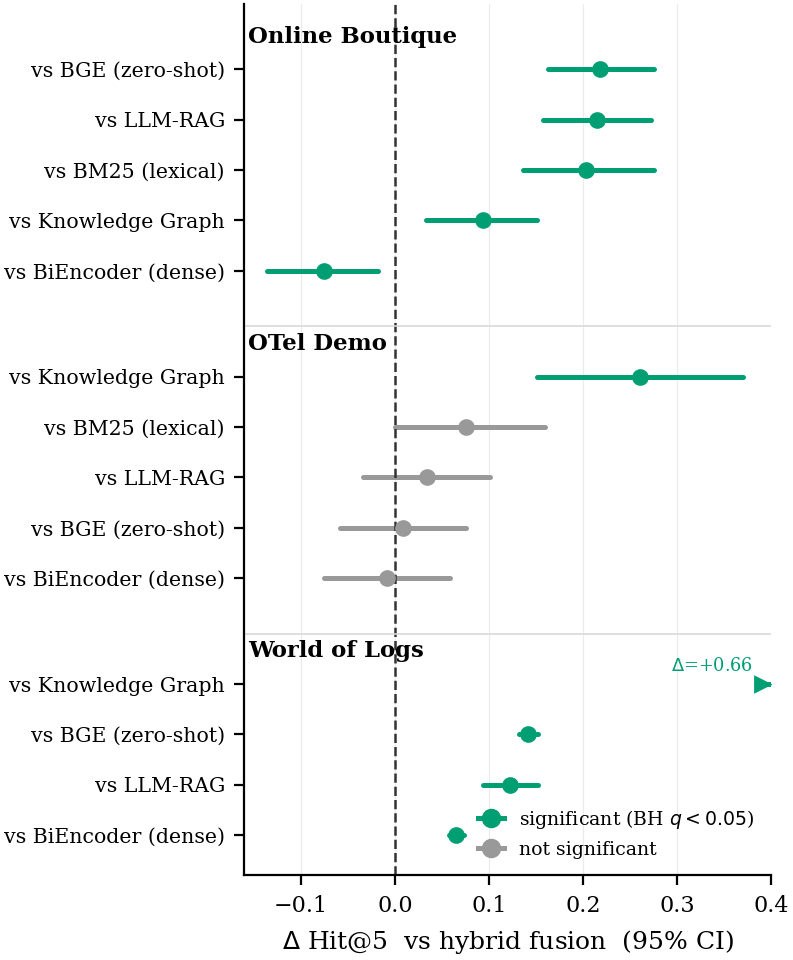
\includegraphics[width=0.82\columnwidth]{figures/fig_significance_forest.png}
\caption{Difference in \hit{5} between hybrid fusion and each alternative (paired
bootstrap, $95\%$ CI; green = significant after Benjamini--Hochberg). Hybrid wins
decisively on real data (WoL) and beats the graph baseline on every dataset; on
the small synthetic corpora it ties or trails the fine-tuned dense retriever.}
\label{fig:forest}
\end{figure}

\subsubsection*{The stricter relation, and what the numbers are worth}
\label{sec:results-strict}

The coarse relation is permissive, and we think the honest way to present it is
alongside both a stricter relation and a reference point for what the scores
mean. Table~\ref{tab:strict} reports every method we have per-query predictions
for under the strict relation, which additionally demands substantial symptom
overlap.

Two calibration facts frame the table. First, the relations differ greatly in how
much of memory they admit: the average query has $288$ relevant items under the
coarse relation ($0.75\%$ of the $38{,}642$-item memory) but only $34.5$ under the
strict one ($0.09\%$). Second, the corresponding expected \hit{5} for a uniformly
random ranker is therefore $0.036$ coarse and $0.0044$ strict. Hybrid retrieval's
$0.970$ and $0.744$ sit $27\times$ and $169\times$ above those references.

Under the strict relation hybrid fusion remains best on all three metrics against
every system we could test pairwise, and the margins survive correction: $+0.038$
\hit{5} over BGE ($95\%$ CI $[+0.025,+0.051]$), $+0.050$ over the cross-encoder
($[+0.038,+0.064]$), and $+0.221$ over our own dense retriever
($[+0.206,+0.237]$), all with Benjamini--Hochberg $q<0.001$. The single exception
is \hit{5} against raw-corpus BM25 ($+0.004$, $[-0.011,+0.019]$, $q=0.54$); that
method's \hit{1} of $0.015$ reflects a degenerate top-rank ordering, and hybrid
beats it on MRR by $+0.271$. The result also holds across \emph{both} held-out
project domains (Kafka~$0.80$, MariaDB~$0.73$).

One result in Table~\ref{tab:strict} deserves emphasis because it cuts against
our own method. Our fine-tuned dense retriever, which is trained against the
coarse relation, is the \emph{largest} loser under the strict one, falling from
$0.905$ to $0.523$ and dropping below every zero-shot embedder. Fusion does not:
it falls from $0.970$ to $0.744$ and stays on top. We read this as evidence that
the evaluation is not simply rewarding methods aligned with the labelling rule
(\S\ref{sec:results-leakage}), since the component most aligned with that rule
degrades the most.

\begin{table}[t]
\centering
\caption{Retrieval on World of Logs under the \emph{strict} relation (coarse
$+$ symptom-token overlap), on the $n{=}4{,}362$ held-out queries that retain a
gold match under it. Best per column in \textbf{bold}. A uniformly random ranker
would score \hit{5}~$0.0044$ here. The fine-tuned dense retriever, trained
against the coarse relation, degrades most; fusion holds up.}
\label{tab:strict}
\footnotesize
\setlength{\tabcolsep}{5pt}
\begin{tabular}{lccc}
\toprule
Method & \hit{1} & \hit{5} & MRR \\
\midrule
\multicolumn{4}{l}{\emph{Prior art, zero-shot}}\\
\quad BGE (dense)          & 0.474 & 0.706 & 0.564 \\
\quad E5 (dense)           & 0.450 & 0.698 & 0.544 \\
\quad TF--IDF (lexical)    & 0.445 & 0.715 & 0.559 \\
\quad BM25 (raw corpus)    & 0.015 & 0.740 & 0.332 \\
\quad Cross-encoder rerank & 0.418 & 0.694 & 0.523 \\
\multicolumn{4}{l}{\emph{Ours}}\\
\quad Dense bi-encoder     & 0.260 & 0.523 & 0.356 \\
\quad Knowledge graph      & 0.016 & 0.036 & 0.023 \\
\quad Hybrid fusion        & \textbf{0.511} & \textbf{0.744} & \textbf{0.602} \\
\bottomrule
\end{tabular}
\end{table}

We isolated the graph's contribution by comparing fusion with and without it. It surfaces correct candidates the
others miss (on $14\%$ of Online Boutique queries it retrieves the right
incident where the dense retriever fails), but in fusion this rarely changes
top-five recall (the $\pm$graph difference is not significant on any dataset).
The graph is therefore a real but marginal contributor: useful for top-rank
precision and coverage, not a driver of \hit{5}.

\subsubsection*{Does the relevance rule leak into the retrievers?}
\label{sec:results-leakage}

The coarse relation is defined on a ticket's Jira \texttt{components} metadata,
and our graph retriever scores candidates partly by component overlap. That
coincidence invites a serious objection: perhaps the headline reflects the
labelling rule rather than retrieval quality. We take it seriously and report
four independent checks, three of which we ran specifically to test it.

\emph{(i) The retrievers never see the field.} The indexed corpus is built from
ticket narrative and pasted log and code blocks only. Sampling $3{,}000$ indexed
memory documents, \emph{none} contains a \texttt{Components} field, and only
$34.6\%$ of gold component names appear anywhere in the indexed text at all, as
incidental prose mentions. On the query side the figure is $15.9\%$. (A legacy
composed-text file in our data release does embed the field verbatim; it is not
what is indexed, and we exclude it from the published bundle to prevent a reader
from reproducing against it by mistake.)

\emph{(ii) The graph's vocabulary barely overlaps the gold vocabulary.} Graph
entities are extracted from ticket text by a language model, not read from
metadata. Over the $38{,}600$ memory extractions the extracted component
vocabulary has $1{,}559$ distinct terms and the gold vocabulary $1{,}101$; they
share $109$, or $9.9\%$ of the gold vocabulary. Roughly nine in ten terms that
define relevance never enter the graph.

\emph{(iii) The graph retriever is the worst system, not the best.} If the rule
leaked through it, it would dominate. It is last under both relations (coarse
\hit{5}~$0.308$, strict $0.036$), and removing it from fusion changes \hit{5}
significantly on no dataset.

\emph{(iv) The component most aligned with the rule degrades the most.} As noted
above, our dense retriever is fine-tuned against the coarse relation and loses
most under the strict one ($0.905\!\rightarrow\!0.523$), while fusion holds up
($0.970\!\rightarrow\!0.744$). An evaluation rigged toward our method would not
behave this way.

None of this makes the coarse relation a measure of diagnostic usefulness, which
it is not (\S\ref{sec:threats}); it addresses only the narrower question of
whether the labelling rule leaks into the systems being compared. We find no
evidence that it does.

\smallskip
\noindent\textbf{How much does the training seed matter?} Retriever fine-tuning
is the only stochastic step in the pipeline (\S\ref{sec:setup-protocol}), so we
quantify its contribution rather than assume it away. Retraining under five
seeds leaves coarse \hit{5} at $0.636\pm0.016$ on Online Boutique and
$0.676\pm0.005$ on OTel Demo (mean $\pm$ sample standard deviation), so the lead
over the zero-shot embedders is not an artifact of a lucky initialization.

Decomposing that variability against the other source, sampling of the test
queries, shows the two datasets behave quite differently. On OTel Demo the seed
standard deviation ($0.005$) is dwarfed by the query-bootstrap standard deviation
($0.044$) and contributes about $1\%$ of the total variance; there, a single run
is defensible. On Online Boutique the two are comparable ($0.016$ versus
$0.026$), with the seed accounting for roughly $28\%$ of the variance, so an
interval computed from query resampling alone understates the true uncertainty.
We therefore report seed-aware intervals, $\sqrt{\sigma^2_{\text{seed}}+
\sigma^2_{\text{sample}}}$, wherever a retrained component is compared.

We note two things about the magnitude. Top-1 is markedly less stable than
top-5 on Online Boutique (\hit{1} spans $0.417$--$0.468$ across seeds, a range of
$0.051$, against $0.039$ for \hit{5}), so single-seed \hit{1} comparisons on the
small corpora deserve particular caution. And the largest full seed-to-seed range
we observe anywhere is $0.039$, against which the real corpus's headline margin
of $+0.065$ \hit{5} over the dense retriever is a factor of $1.7$ larger.

\subsection{RQ2: End-to-End Triage and Graceful Degradation}
\label{sec:results-rq2}

Table~\ref{tab:agent} reports the full end-to-end system. The headline is
robustness across evidence regimes: the \emph{same} system, with no
reconfiguration, retrieves strongly whether it has complete telemetry or only text,
reaching \hit{5}~$0.96$ on the real, text-only incidents (essentially realizing the
hybrid retriever's quality end to end) and $0.76$ on the fully instrumented
synthetic systems.

Duplicate suppression fires where there are duplicates to suppress, and we report
it as a rate rather than as pages per incident, which our harness makes $1.0$ by
construction. On the real corpus, $3{,}061$ of $10{,}566$ would-be pages
($29.0\%$) are folded into an incident already raised. The telemetry corpora give
it far less to do ($5.3\%$ and $0.9\%$), since their scenarios are short and
rarely span many consecutive ticket-worthy windows; the mechanism is therefore
exercised meaningfully only on the real corpus, and we do not claim it as
validated on the synthetic ones.

Triage accuracy tells a different story across regimes. On the telemetry datasets
the system clears the majority-class baseline by a useful margin ($0.841$ against
$0.784$, and $0.846$ against $0.725$). On the real corpus it reaches $0.506$
against a $0.506$ baseline, i.e.\ no better than always predicting the majority
class. We say this plainly: our own end-to-end triage on real incidents carries
no usable signal either, which is consistent with, not an exception to, the
reframing in \S\ref{sec:results-rq4}.

One might suspect this is an artifact of page suppression, which re-labels a
suppressed window \emph{borderline}, a class the binary resolution-derived gold
cannot match. It is not. The harness scores triage on the pre-suppression
decision precisely to avoid charging a paging action as a triage error, and the
effect is verifiable: a configuration with suppression disabled, which emits no
borderline decisions at all, classifies exactly the same $6{,}769$ of $13{,}388$
windows correctly as the configuration that suppresses $3{,}061$ pages. The
$0.506$ is therefore a genuine absence of signal, not a scoring artifact.

\begin{table}[t]
\centering
\caption{End-to-end system (RQ2) and the cost saved by capability gating (RQ3),
per dataset. Triage accuracy is reported against the majority-class baseline,
which it does not beat on the real corpus. Duplicate suppression is given as the
share of would-be pages folded into an existing incident; we do not report pages
per incident, which is $1.0$ by construction in our harness and therefore
uninformative. Cost saving is an \emph{estimated} counterfactual: gate decisions
priced with a fixed per-skill cost model (\S\ref{sec:results-rq3}), not a
measured wall-clock comparison.}
\label{tab:agent}
\footnotesize
\setlength{\tabcolsep}{5pt}
\begin{tabular}{lccc}
\toprule
 & Online Boutique & OTel Demo & World of Logs \\
\midrule
\hit{1}                        & 0.689 & 0.647 & 0.859 \\
\hit{5}                        & 0.758 & 0.756 & 0.963 \\
MRR                            & 0.714 & 0.688 & 0.902 \\
Triage accuracy                & 0.841 & 0.846 & 0.506 \\
\quad\emph{majority baseline}  & \emph{0.784} & \emph{0.725} & \emph{0.506} \\
Would-be pages suppressed      & 5.3\% & 0.9\% & 29.0\% \\
\midrule
Cost saved (gating, estimated) & 40\%  & 63\%  & 78\% \\
\bottomrule
\end{tabular}
\end{table}

\subsection{RQ3: The Cost of Adaptive Execution}
\label{sec:results-rq3}

What does the capability-gated controller buy? Running only the steps the
evidence supports, and escalating expensive steps only under uncertainty,
reduces per-window cost by $40\%$, $63\%$, and $78\%$ on the three datasets
relative to a cascade that runs everything (Table~\ref{tab:agent}).

We are precise about what that figure is and is not. The \emph{counts} are
measured: we log per window which skills ran and which a gate skipped
($75{,}334$ invocations and $31{,}734$ gate skips on the real corpus). The
\emph{per-call unit costs} are modelled, from a fixed table released with the
artifact. The reported percentage is counts $\times$ modelled units, so calling
it a measured wall-clock reduction, as our earlier phrasing did, overstates it.

The natural objection is that the conclusion then rests on the cost table. It
does not, and the reason is structural. Every gated skill sits behind the
\emph{same} escalation gate, so each is skipped at nearly the same rate; the
saving therefore approximates that gate's closure rate almost independently of
what the individual skills cost. Recomputing the entire saving with each skill's
\emph{measured} mean duration as its unit cost, instead of the modelled one,
gives $79.0\%$ against the modelled $77.9\%$, a difference of $1.1$ points, even
though the table misprices individual skills badly (it overstates query
reformulation by three orders of magnitude and understates the peer-incident
lookup, the only step doing real I/O, by $68\times$). Varying the verifier's
assumed per-call cost between $0.5\times$ and $2\times$ moves the real-corpus
figure not at all, since that skill is disabled there.

What the figure does \emph{not} capture is equally important: this evaluation
harness replays precomputed predictions, so its measured end-to-end wall-clock
($43$\,ms per window) is the cost of replaying a decision, not of making one. We
therefore report cost as an explicitly modelled counterfactual rather than as a
deployment measurement, and treat the gate-closure rates as the quantity the
result actually rests on. Those rates are what differ across datasets: the $78\%$
on the real corpus reflects reformulation being skipped on $10{,}566$ of
$13{,}376$ windows, and the telemetry figures reflect the evidence tools being
skipped on $41\%$ and $65\%$. The saving does not "grow with scale" so much as
track how often each deployment's dominant gate closes.

This thrift costs no accuracy: an ablation that
removes each component in turn moves \hit{1} by at most $0.012$, and sweeping the
evidence-gathering budget leaves \hit{5} unchanged. The same measurements carry a candid message: no single component is load-bearing, so the heavyweight evidence-gathering tools add little measurable \hit{} gain here; they keep cost low by running only when cheaper steps are unsure, and their headroom is bounded by how often retrieval is already correct.

\smallskip
\noindent\textbf{Where the gate thresholds sit.} Because the escalation decision
is driven by a threshold on $\mathrm{maxconf}$ (Eq.~\ref{eq:maxconf}), its value
deserves a sensitivity analysis rather than an assertion. Using the per-window
counterfactual between the cheap-path-only and full-stack configurations, we
sweep a unified escalation threshold over the realized confidence distribution on
the real corpus (Table~\ref{tab:threshold}). Escalation is worth $+0.059$ \hit{5}
in aggregate ($0.904\!\rightarrow\!0.963$), but the curve saturates early: a
threshold of $0.477$ already reaches the full-escalation quality of $0.963$ while
escalating three quarters of windows, and $0.362$ retains $0.935$ while escalating
only a quarter. The shipped $0.5$ is thus on the saturated plateau, buying no
additional quality over $0.477$ at a higher escalation rate. On the telemetry
datasets the sweep is flat at every threshold, consistent with the finding above
that the expensive path never changes their rankings.

\begin{table}[t]
\centering
\caption{Escalation-threshold sensitivity on World of Logs ($n{=}5{,}150$). A
window escalates when its cheap-path confidence falls below the threshold.
Quality saturates well before the shipped operating point.}
\label{tab:threshold}
\footnotesize
\setlength{\tabcolsep}{5pt}
\begin{tabular}{cccl}
\toprule
Threshold & Windows escalated & \hit{5} & \\
\midrule
$0.000$ & \phantom{0}0.0\% & 0.904 & (never escalate) \\
$0.293$ & \phantom{0}5.0\% & 0.911 & \\
$0.362$ & 25.0\% & 0.935 & \\
$0.400$ & 41.8\% & 0.955 & \\
$0.450$ & 61.0\% & 0.963 & \\
$0.477$ & 75.0\% & 0.963 & cheapest to match full escalation \\
$0.500$ & 85.4\% & 0.963 & shipped operating point \\
$0.600$ & 100.0\% & 0.963 & (always escalate) \\
\bottomrule
\end{tabular}
\end{table}

\smallskip
\noindent The ablation isolates one capability that sits apart from retrieval rank,
\emph{novelty detection}: removing the novelty-composition step leaves \hit{5}
unchanged but drops recall of novel, no-precedent incidents from $0.54$ to $0$ on
Online Boutique, so the step is load-bearing for flagging failures with no
precedent even though it never moves top-five retrieval. On the text-only real
corpus this flag is confounded with ordinary retrieval uncertainty (weakening
retrieval only makes more windows look novel), so we report novelty on the
synthetic telemetry data alone.

\begin{figure*}[t]
\centering
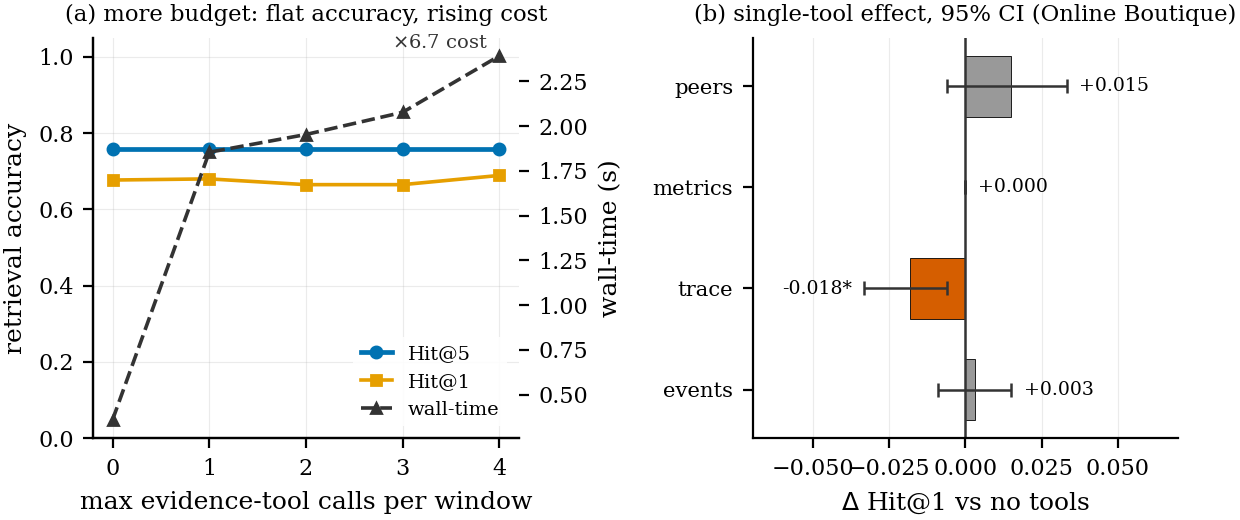
\includegraphics[width=.8\textwidth]{figures/fig_adaptive_execution.png}
\caption{Adaptive execution on the fully-instrumented Online Boutique system
(RQ3). (a)~Raising the evidence-gathering budget leaves retrieval accuracy
unchanged (\hit{5} flat at $0.76$; \hit{1} within a $0.024$ band) while wall-clock
time grows $6.7\times$: more budget buys latency, not accuracy. (b)~Single-tool
effect on \hit{1} with $95\%$ paired-bootstrap confidence intervals ($1{,}000$
resamples, the same procedure as Fig.~\ref{fig:forest}); $*$ marks an interval
excluding zero. \emph{No evidence tool has a demonstrable benefit}: the
peer-incident lookup, the largest positive point estimate, is
$+0.015$ with CI $[-0.006,+0.033]$. Only the extended-trace reader has a
demonstrable effect and it is \emph{harmful} ($-0.018$, CI $[-0.033,-0.006]$),
and only when it runs alone: added alongside the peer lookup the effect falls to
$-0.003$ (CI $[-0.009,+0.000]$, n.s.). On OTel Demo and World of Logs every tool
effect is identically $0.000$. The controller's value is therefore to invoke
these tools only when cheaper steps are unsure, not to add accuracy.}
\label{fig:adaptive}
\end{figure*}

\subsection{RQ4: Synthetic Versus Real, and What It Reveals}
\label{sec:results-rq4}

Our most consequential finding concerns the triage \emph{classification} task
that dominates synthetic benchmarks, deciding whether a window is ticket-worthy
at all. On synthetic data it is trivially easy: standard classifiers over the
telemetry features reach a near-perfect area under the precision--recall curve
(ROC area $1.00$) and are well calibrated.

Real incidents carry no telemetry features, so the comparison must be made on
the input that corpus actually has, its text. Under the identical
leave-domain-out protocol and five seeds, a TF--IDF linear model reaches ROC
area $0.601$ ($95\%$ CI $[0.592,0.611]$), gradient boosting over a truncated-SVD
projection $0.583$, and logistic regression $0.572$. The intervals exclude
$0.50$, so real-incident text does carry signal, but the task retains only a
small fraction of what injected telemetry offers, and at the operating threshold
the gain over the majority-class baseline ($0.506$) is slight. The near-perfect
synthetic number is thus an artifact of fault injection, where active faults are
separable from baselines by construction, rather than evidence that
ticket-worthiness is an easy prediction on real, engineer-written tickets. We further confirm that the synthetic signal is
genuine rather than memorized: on Online Boutique we inject \emph{orphan} faults,
real ticket-worthy failures deliberately left with no matching ticket in memory, and
the triage classifiers flag them as reliably as the reported faults (recall gap
within $5$ points, and $1.00$ versus $1.00$ for the gradient-boosted model), so the
near-perfect synthetic number reflects fault-versus-baseline separability, not
memorization of which incidents carry tickets. This check is informative only there:
the other telemetry set contained no orphan faults, and on the real corpus triage is
already weak.

The real-data conclusion is not an artifact of how we binarize the three-way
label. Dropping the ambiguous \emph{borderline} class and classifying
ticket-worthy against noise alone raises the best text model to ROC area $0.704$
($95\%$ CI $[0.688,0.721]$) on $8{,}024$ held-out issues, still far below the
synthetic $1.00$ and still at the majority-class accuracy ($0.844$). Both
binarizations agree: real-incident text carries measurable but weak
ticket-worthiness signal.

This reframes how operational triage should be measured: the part that looks solved on synthetic data does not transfer, while the part that does (retrieving which past incident a live one resembles) is where the real headroom lies, and where our system is strongest.

Because the real dataset's matches are inferred rather than human-labelled, we
probed them with an LLM-as-judge. Asked to rate each gold match against a control,
the judge separates the two on every dataset, most sharply on the real incidents
(a gold-versus-control gap of $1.24$ on a five-point scale, versus $0.34$--$0.47$
on synthetic). The same run, however, qualifies what that gap establishes: only
$6.3\%$ of coarse-gold matches are rated $4$ or $5$, against $0\%$ of controls. So
the judge finds the relation clearly non-random, but it does \emph{not} find most
coarse-gold pairs to be strongly related. Together with the controls being
uniformly sampled, and therefore easy, this check should be read as evidence that
the coarse relation captures topical relatedness, not that it identifies the
prior incident an engineer would most want. We report the strict relation
(\S\ref{sec:results-strict}) for that reason, and a human study remains the
right instrument (\S\ref{sec:threats}).
% === Discussion ===
\section{Discussion}
\label{sec:discussion}

\noindent\textbf{Triage-as-classification is a weak yardstick.} The task most
automated-triage work optimizes, deciding whether a window is ticket-worthy at
all, is saturated where it is usually measured and barely learnable where it
matters: on injected faults an active fault is separable from a healthy baseline
almost by construction, while on real engineer-filed tickets every classifier we
tried sat at chance (\S\ref{sec:results-rq4}). Strong synthetic triage numbers
therefore certify the dataset, not the method, and a system tuned to maximize them
optimizes a quantity that does not transfer. The problem worth solving is the one
that does: recognizing \emph{which} past incident a live one resembles, far from
saturated and where our gains come from.

\noindent\textbf{Method conclusions flip with scale and realism.} Had we evaluated
retrieval only on the synthetic corpora, as is common, we would have concluded
that fusing retrievers is useless, even mildly harmful, and shipped a single dense
model. On the real corpus, an order of magnitude larger and spread across two
dozen projects, the same fusion is decisively best (Figure~\ref{fig:forest}): a large, diverse
memory creates blind spots that complementary retrievers cover, while in a small,
homogeneous one a single retriever dominates and weaker signals only add noise. With
only three corpora we cannot fully disentangle scale from diversity, so we claim only
per dataset: fusion is significantly best on the large, heterogeneous real corpus and
ties or trails the dense retriever on the small synthetic ones. Retrieval comparisons thus need realistic scale \emph{and}
diversity before their conclusions can be trusted, one reason we release
real-scale data alongside the synthetic.

\noindent\textbf{Robustness comes from asking ``does this step help \emph{here}?''}
The right action depends on the deployment. The language-model verifier improves
synthetic triage yet is net-negative on real text and is switched off there; the
retrieval-augmented language model never beats the domain-tuned retriever whose
candidates it re-reads. A system that hard-codes such components pays for them
everywhere and is hurt where they misfire. Our controller instead treats both
\emph{what evidence is present} and \emph{whether an expensive step helps} as
per-window decisions, letting one implementation run from full telemetry down to
bare text, suppress duplicate pages, and shed $40$--$78\%$ of per-window cost with no
loss in accuracy (Figure~\ref{fig:adaptive}). Large language models are not a default win in this
domain; the leverage lies in a controller that invokes them selectively and
measures their effect.

\noindent\textbf{The system's contribution is efficiency and reach, not peak
accuracy.} The full system does not beat the best single retriever on raw hit
rate; it \emph{matches} that quality at a fraction of the budget and keeps
working when most of the evidence disappears. In real operations, where
instrumentation is uneven, alert volume is punishing, and compute is metered,
peak-quality retrieval when warranted, a lightweight path when not,
and roughly one alert per incident are precisely what makes a triage
assistant deployable.

%\noindent\textbf{Open problems.} Two gaps frame future work. First, the knowledge graph supplies correct candidates the other retrievers miss yet moves top-five recall little; richer relational extraction or a learned graph matcher, rather than entity overlap, may convert that latent signal into measured gains. Second, our real-world data is text only while our telemetry-rich data is synthetic: the open frontier is real telemetry paired with real, human-written tickets at scale. The datasets, harness, and baselines we release lower the barrier; \S\ref{sec:threats} discusses the limitations that temper these conclusions.

% === Threats to Validity ===
\section{Threats to Validity}
\label{sec:threats}

Several threats temper our claims. The principal one is \emph{external}: our
telemetry-rich datasets are synthetic while our real dataset is text only, so
on-demand evidence-gathering is exercised only on injected faults and we
do not claim it transfers to production telemetry; the open-source Apache
incidents and two demonstration applications are not a representative sample of
all deployments. On \emph{construct} validity, the real dataset has no
ground-truth answer key, so matches are inferred from project, component, and
symptom overlap; we mitigate this with an LLM-as-judge check that separates true
matches from random controls on every dataset (\S\ref{sec:results-rq4}), report
both a coarse and a strict relation, and release a human-annotation kit, but the
labels remain a proxy rather than a multi-annotator study. For \emph{internal}
validity, time-aware visibility and held-out fault families and project domains
prevent leakage of future or training information, though only the costly
real-data retriever is trained on a single seed (the two telemetry retrievers are
stable across three seeds, \S\ref{sec:results-rq1}), which we report.
Finally, for \emph{conclusion} validity, every difference is tested with a paired
bootstrap corrected for false discovery, and we report negative and mixed results,
such as fusion's lack of benefit on small corpora and triage's collapse on real
data, rather than reporting only favorable comparisons.

% === Conclusion ===
\section{Conclusion and Future Work}
\label{sec:conclusion}

Incident triage often relies on analogy to previously resolved failures. We
built \sys, a capability-aware system that retrieves similar incidents by fusing
dense, sparse, and graph signals, adapts its reasoning steps to the evidence
available in each window, and suppresses duplicate pages across an incident's
lifetime. Across fully instrumented synthetic services and real Apache Jira
incidents, hybrid retrieval returns an inferred relevant prior incident within
the top five results for $97\%$ of real-corpus queries, improving top-five
retrieval over dense, lexical, graph, and LLM baselines. Capability gating
preserves retrieval quality while reducing cost by up to $78\%$ and degrading
gracefully to text-only operation. Our main evaluation lesson is that
ticket-worthiness classification is nearly solved on injected faults but fails
under text-only, resolution-derived real-incident labels; incident-memory
retrieval is therefore a more transferable target for operational triage.

Future work should evaluate \sys on production telemetry paired with
human-written incident tickets, validate incident similarity through
multi-annotator judgments from engineers, and improve graph retrieval through
richer relation extraction or learned graph matching.

\section*{Data Availability}

All source code, the evaluation harness, the collected telemetry datasets, and
the complete result set are released to support reproduction. The datasets are
available at Zenodo, \url{https://zenodo.org/records/21096887}
(DOI~10.5281/zenodo.21096887), and the source code and evaluation harness at
\url{https://zenodo.org/records/21096898}
(DOI~10.5281/zenodo.21096898). Only the derived Apache-project Jira subset of the
World of Logs corpus is redistributed there, under CC~BY~4.0; the full corpus is
available from its original authors under its own terms.

\clearpage
\balance
\bibliographystyle{IEEEtran}
\bibliography{refs}

\end{document}



